\section{Feature Selection}
Özellik seçimi, veri setindeki en önemli özellikleri belirleyerek, modelin daha iyi performans göstermesini sağlayan bir süreçtir. Bu süreçte, gereksiz veya düşük önemli özelliklerin filtrelenmesi ve modelin daha iyi genelleme yapabilmesini sağlayacak şekilde veri setinin basitleştirilmesi amaçlanır. Doğru özelliklerin seçilmesi, modelin doğruluğunu artırabilir ve gereksiz hesaplama maliyetlerini azaltabilir.

\begin{figure}[h]
    \centering
    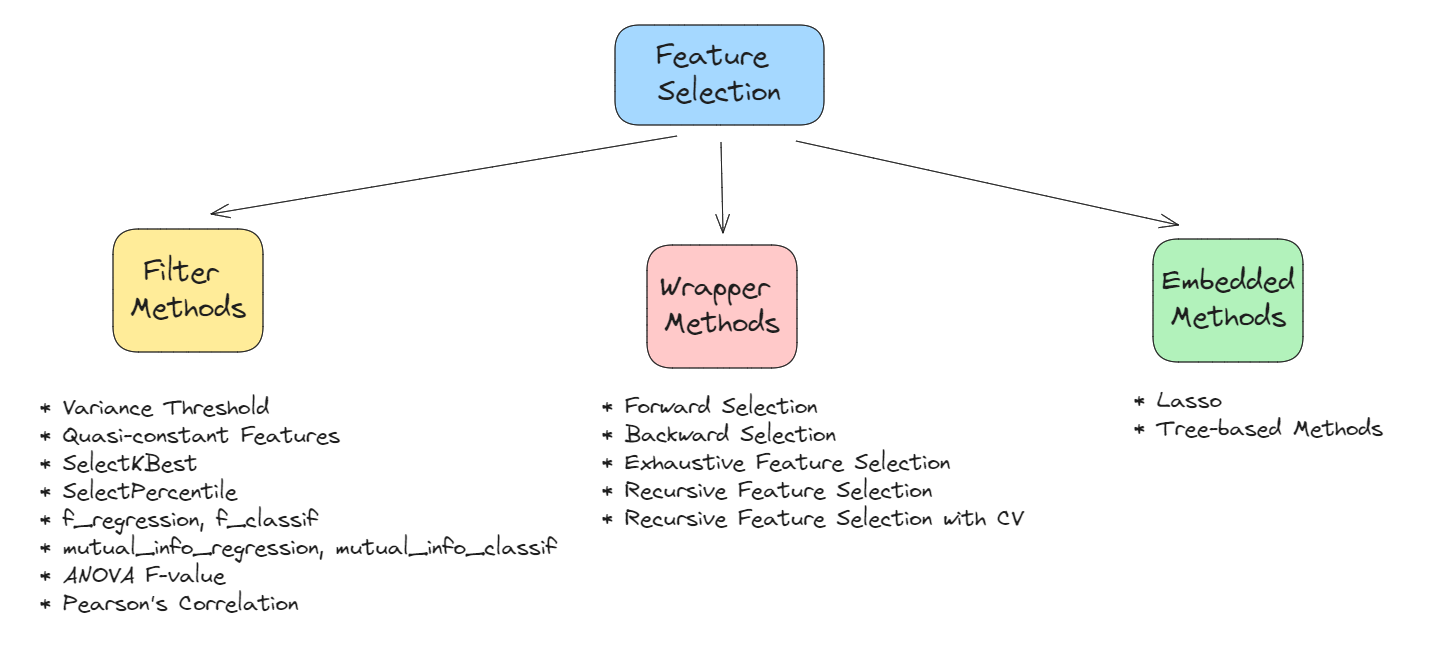
\includegraphics[width=1\textwidth]{images/feature_selection_methods.png}
    \caption{Özellik seçimi metodları.}
    \label{fig:enter-label}
\end{figure}

\newpage

\subsection{Filter Methods (Filtre Yöntemleri)}
Filtre yöntemleri bir ön işleme adımı olarak kullanılır. Özelliklerin seçimi herhangi bir makine öğrenimi algoritmasından bağımsızdır. Bunun yerine, özellikler, sonuç değişkeniyle olan korelasyonlarına yönelik çeşitli istatistiksel testlerdeki puanlarına göre seçilir. Wrapper Methods (Sarmalayıcı Yöntemler)'den daha düşük tahmin performansı verirler. Hızlı bir tarama ve alakasız özelliklerin çıkarılması için çok uygundurlar.

\textbf{Variance Threshold (Varyans Eşiği):} Varyansı belirli bir eşiği karşılamayan tüm özellikleri kaldırır. Default olarak tüm sıfır varyanslı özellikleri kaldırır.

\begin{lstlisting}[language=Python]
from sklearn.feature_selection import VarianceThreshold
vt = VarianceThreshold(threshold=0).fit(X_train)

vt.get_support()
\end{lstlisting}

\textbf{Quasi-constant Features (Yarı sabit özellikler):} Yarı sabit özellikler, veri kümesindeki gözlemlerin büyük çoğunluğu için aynı değeri gösteren özelliklerdir. Bu özellikler, bir makine öğrenimi modelinin bir hedefi ayırt etmesine veya tahmin etmesine olanak tanıyan çok az bilgi sağlar. Ancak istisnalar da olabilir.

\begin{lstlisting}[language=Python]
from sklearn.feature_selection import VarianceThreshold
vt = VarianceThreshold(threshold=0.01).fit(X_train)

vt.get_support()
\end{lstlisting}

\textbf{SelectKBest:} Özellikleri en yüksek k puana göre seçer. Beraber Chi-square testi yapılabilir.

\begin{lstlisting}[language=Python]
from sklearn.feature_selection import SelectKBest, chi2
X_new = SelectKBest(chi2, k=3).fit_transform(X, y)
X_new.shape
\end{lstlisting}

\textbf{SelectPercentile:} En yüksek puanların yüzdelik dilimine göre özellikleri seçer.

\begin{lstlisting}[language=Python]
from sklearn.feature_selection import SelectPercentile, chi2
X_new = SelectPercentile(chi2, percentile=5).fit_transform(X, y)
X_new.shape
\end{lstlisting}

Regresyon problemleri için: f\_regression, mutual\_info\_regression
\begin{lstlisting}[language=Python]
f_value = f_regression(X_train, y_train)

for feature in zip(X_train.columns, f_value[0]):
	print(feature)

mi_score = mutual_info_regression(X_train, y_train)
for feature in zip(X_train.columns, mi_score):
	print(feature)
\end{lstlisting}

Sınıflandırma problemleri için: chi2, f\_classif, mutual\_info\_classif
\begin{lstlisting}[language=Python]
f_value = f_classif(X_train, y_train)

for feature in zip(X_train.columns, f_value[0]):
	print(feature)

mi_score = mutual_info_classif(X_train, y_train)
for feature in zip(X_train.columns, mi_score):
	print(feature)
\end{lstlisting}

F-testine dayalı yöntemler iki rastgele değişken arasındaki doğrusal bağımlılık derecesini tahmin eder. Karşılıklı bilgi yöntemleri (mutual\_ ile başlayanlar) her türlü istatistiksel bağımlılığı yakalayabilir ancak parametrik olmadıkları için doğru tahmin için daha fazla örneğe ihtiyaç duyarlar.

\begin{enumerate}
    \item \textbf{Information Gain (Karşılıklı Bilgi):} Bir özelliğin varlığının/yokluğunun hedef hakkında doğru tahminde bulunmaya ne kadar katkıda bulunduğunu ölçer. Bu değişkenlerden birini bilmenin diğer hakkıdaki belirsizliği ne kadar azalttığını ölçer. Örneğin X-Y bağımsızsa birini bilmenin diğeri hakkında bilgi vermez. Böylece information gain = 0'dır.
    \item \textbf{Fisher Score:} Negatif olmayan her özellik ve sınıf arasındaki ki-kare istatistiklerini hesaplar. Özellikler kategorik ise chi2 kullanılır.
    \item \textbf{ANOVA F-value:} Özellikler nicel ise her bir özellik ile hedef arasındaki ANOVA F-değeri hesaplanır. F-değeri, sayısal özelliği hedefe göre gruplandırdığımızda, her bir grubun ortalamalarının önemli ölçüde farklı olup olmadığını hesaplar.
    \item \textbf{Pearson Correlation:} Korelasyon, 2 veya daha fazla değişkenin doğrusal ilişkisinin bir ölçüsüdür. Korelasyon sayesinde bir değişkeni diğerinden tahmin edebiliriz. İyi değişkenler hedef değişkenle yüksek oranda ilişkilidir. Değişkenler hedef değişkenle ilişkili olmalı fakat kendi aralarında ilişkisiz olmalıdır. Eğer öyleyse, korelasyonlu olanlardan sadece birini tutmamız ve diğerlerini bırakmamız gerekir.
\end{enumerate}

\newpage

\subsection{Wrapper Methods (Sarmalayıcı Yöntemler)}
Sarmalayıcı yöntemlerde, özelliklerin bir alt kümesini kullanmaya ve bunları kullanarak bir model eğitmeye çalışılır. Önceki modelden çıkardığımız çıkarımlara dayanarak, alt kümeye özellik eklemeye veya çıkarmaya karar verilir.

\textbf{Forward Selection:} Modelde hiçbir özellik olmadan başlanan iteratif bir yöntemdir. Her bir iterasyonda, yeni bir değişken eklenmesi modelin performansını iyileştirmeyene kadar modeli en iyi iyileştiren özelliği eklemeye devam eder.

\begin{lstlisting}[language=Python]
from mlxtend.feature_selection import SequentialFeatureSelector

sfs = SequentialFeatureSelector(RandomForestRegressor(), 
								   k_features=10, 
								   forward=True, 
								   floating=False, 
								   verbose=2,
								   scoring='r2',
								   cv=5)

sfs = sfs.fit(np.array(X_train), y_train)
sfs.k_feature_idx_
\end{lstlisting}

\textbf{Backward Selection:} Tüm özelliklerle başlanır ve her iterasyonda modelin performansını artıran en az anlamlı özellik kaldırılır. Bu işlem, özelliklerin kaldırılmasında herhangi bir iyileşme gözlenmeyene kadar tekrarlanır.

\begin{lstlisting}[language=Python]
from mlxtend.feature_selection import SequentialFeatureSelector

sfs = SequentialFeatureSelector(RandomForestRegressor(), 
								   k_features=10, 
								   forward=False, 
								   floating=False, 
								   verbose=2,
								   scoring='r2',
								   cv=5)

sfs = sfs.fit(np.array(X_train), y_train)
sfs.k_feature_idx_
\end{lstlisting}

\textbf{Exhaustive Feature Selection:} Bir algoritma için belirli bir performans metriğini optimize ederek tüm olası özellik alt kümeleri arasından en iyi özellik alt kümesi seçilir.\newline
\textbf{Recursive Feature Elimination:} En iyi performans gösteren özellik alt kümesini bulmayı amaçlayan açgözlü bir optimizasyon algoritmasıdır. Tekrar tekrar modeller oluşturur ve her iterasyonda en iyi veya en kötü performans gösteren özelliği bir kenarda tutar. Tüm özellikler tükenene kadar kalan özelliklerle bir sonraki modeli oluşturur. Daha sonra özellikleri eleme sırasına göre sıralar.\newline
\textbf{Recursive Feature Elimination with CV (RFECV):} 0 ile N özelliği yinelemeli olarak kaldırarak tahmin edici için en iyi özellik alt kümesini seçer.

\newpage

\subsection{Embedded Methods (Gömülü Yöntemler)}
Lasso Regression: Lasso regresyonu, katsayıların büyüklüğünün mutlak değerlerine eşdeğer bir ceza ekleyen bir L1 düzenlemesi gerçekleştirir. L1, bazı katsayıları sıfıra kadar küçültebilen bir özelliğe sahiptir. Bu nedenle, bu özellik modelden çıkarılabilir.

\begin{lstlisting}[language=Python]
from sklearn.feature_selection import SelectFromModel
sel_ = SelectFromModel(Lasso(alpha=100))
sel_.fit(scaler.transform(X_train), y_train)
sel_.get_support()
\end{lstlisting}

Tree-based Methods: Ağaç modellerinin içerisindeki "feature\_importances\_" özelliği ile yapılır.
\begin{lstlisting}[language=Python]
rf = RandomForestClassifier().fit(X_train, y_train)
rf.feature_importances_
\end{lstlisting}

\newpage

\subsection{MAPIE (Model Agnostic Parameter Importance Estimation)}
Modelin türünden bağımsızdır.

\newpage